\documentclass[11pt,a4paper]{article}
\usepackage{fullpage}
\usepackage[utf8]{inputenc}
\usepackage{amsmath}
\usepackage{subcaption}
\usepackage{graphicx}
\usepackage{subfig}
\usepackage{url}

\title{Register allocation for quantum computing}
\author{working draft}

\begin{document}

\maketitle

\section{Introduction}

With the recent introduction of cloud access to quantum computer prototypes,
experimental quantum computing (QC) is now available to a wide community.
For instance, the IBM Quantum Experience program\footnote{\url{http://research.ibm.com/ibm-q/}} lets users submit experiments based on either a visual circuit representation or a gate-level language based on MIT Quantum Assembler (QASM) syntax \cite{Cross17,Svore06}.
However, the level of abstraction offered by quantum circuits is low, and circuits need to obey machine-specific constraints.
Manual mapping and tuning of QC algorithms in QASM is tedious and error-prone.

To compound the issue, today's quantum computer prototypes have tight resource constraints. For instance, the IBM 5Q computer supports at most 5 qubits with limited connectivity. In addition, decoherence effects severely constrain the execution time. Though quantum error-correcting codes may mitigate the decoherence issue, current hardware do not provide enough resources for realistic QEC \cite{Cross17}.
The longer a quantum program runs, the more it is susceptible to noise. Minimizing runtime is crucial as the accuracy of the results depends on it.
% higher-level languages~\cite{Unruh06}
Thus, compilation of quantum circuits demands extremely accurate compiler optimization.

\section{Problem statement}

The issue we address in this work is the efficient mapping of a generic quantum circuit on an actual quantum computer that has limited connectivity.
Our objective is to minimize the complexity of the resulting circuit (based on some metric: depth, time, or gate count?)

\begin{figure}[htb]
\centering
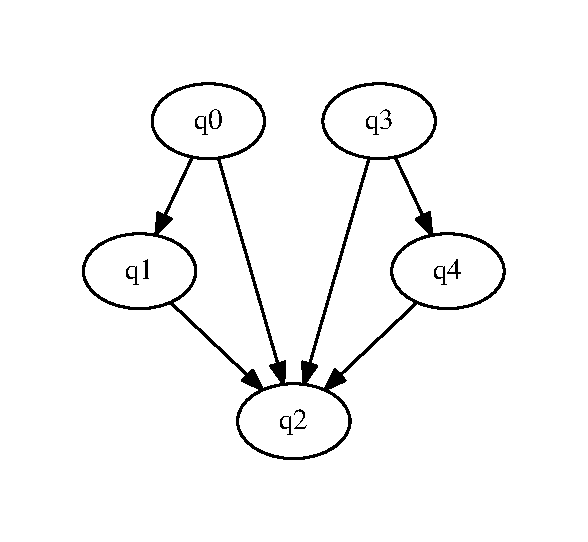
\includegraphics[scale=.5]{fig/ibm5q}
\caption{Connectivity diagram of the IBM 5Q computer}
\label{fig:topology}
\end{figure}

\begin{figure}[htb]
\subcaptionbox{High-level circuit\label{fig:highlevel}}{
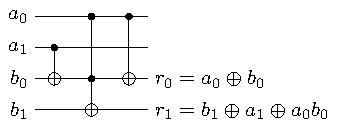
\includegraphics[scale=1]{fig/adder}
}
\subcaptionbox{Low-level circuit\label{fig:lowlevel}}{
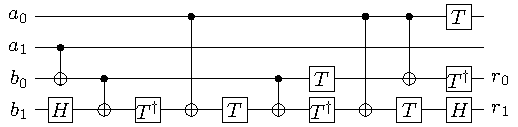
\includegraphics[scale=1]{fig/adder_toffoli}
}
\caption{Adder circuit example}
\label{fig:adder}
\end{figure}

\paragraph{Motivating example: Mapping a 2-bit adder circuit}
In this example, we consider the IBM 5Q computer which supports 5 qubits, with restrictions on which qubit can interact with which.
Figure \ref{fig:topology} shows the topology of this machine as a directed graph. Graph nodes are qubits, and edges denote possible interactions between qubits with CNOT gates.

We want to map to this architecture the high-level circuit of Figure \ref{fig:highlevel}, which implements modulo-4 addition of two numbers by using two CNOT and one Toffoli gate.
As the Toffoli gate is not supported natively on this computer, we must first transform the circuit by substituting a library implementation for the Toffoli gate. After algebraic simplifications, we obtain the circuit of Figure \ref{fig:lowlevel}.
%Invalid interactions.

Interactions between qubits of the low-level circuit of Figure \ref{fig:lowlevel} are represented on the graph of Figure \ref{fig:adder_interact}.
To implement our circuit on the computer, we need to map the logical qubits $a_0, a_1, b_0, b_1$ used by the circuit to the physical qubits $q_0 \dots q_4$ offered by the machine.
It is equivalent to finding an embedding of the interaction graph of the application within the connectivity graph of the machine.
However, such embedding does not exist in our example. Indeed, $b_0$ has two incoming edges and one outgoing edge, unlike any of the nodes of Figure \ref{fig:topology}.
This means the program cannot be readily implemented on the 5Q computer.

Instead, some program transformations are needed first to allow the interaction graph to be embedded in the connectivity graph.
Figure \ref{fig:adder_reverse} presents an equivalent circuit produced by reversing the direction of CNOT gates between $b_0$ and $b_1$, inserting Hadamard gates and optimizing out redundant Hadamard gates.
This new circuit can now be implemented on the quantum computer using for instance $q_3, q_0, q_2, q_4$ as $a_0, a_1, b_0, b_1$, respectively.
Our goal is to automate these transformations by proposing a register allocator for quantum circuits.

\begin{figure}[htb]
\centering
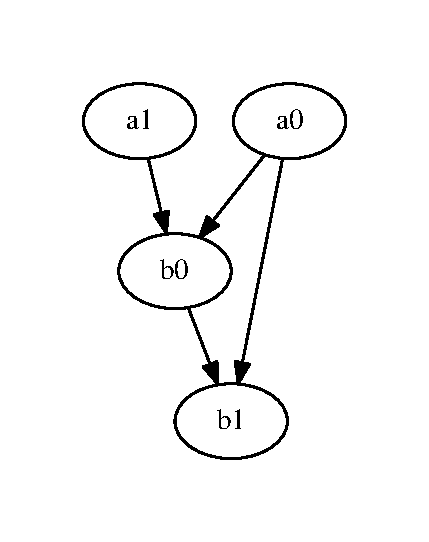
\includegraphics[scale=.5]{fig/adder_interact}
\caption{Interactions between qubits of the adder example}
\label{fig:adder_interact}
\end{figure}

\begin{figure}[htb]
\centering
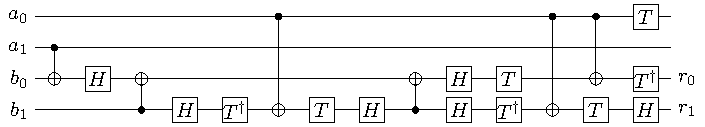
\includegraphics[scale=1]{fig/adder_reverse}
\caption{Adder circuit that obeys machine constraints}
\label{fig:adder_reverse}
\end{figure}

\paragraph{Inputs}
\begin{itemize}
\item A description of the machine topology as a directed graph. Vertices represent physical qubits, and edges represent possible interactions between qubits.
\item A reversible quantum circuit following the quantum gate abstraction. Involves logical qubits.
Ends by measurements of up to $n$ qubits to $n$ classical bits.
\end{itemize}

\paragraph{Outputs}
\begin{itemize}
\item A mapping of physical qubit measurements to logical qubit measurements.
\item A quantum circuit that follow the constraints set by the machine topology.
\end{itemize}

\paragraph{Allowed transformations}
\begin{itemize}
\item CNOT reversal. Emulation of a CNOT between $q_a$ and $q_b$ controlled by $q_a$ using a CNOT from $q_b$ to $q_a$ (controlled by $q_b$) and 2 extra levels of Hadamard gates, as shown on Figure \ref{fig:reverse}. Allows the mapping of ``backward'' edges on the machine connectivity graph at the cost of extra gates.
\item SWAP. Exchanges two qubits $q_a$ and $q_b$, as shown on Figure \ref{fig:swap}. Cost: 3 CNOT and 2 levels of Hadamard gates (assuming one-way connectivity). Allows the migration of logical qubits across physical qubits to obey connectivity constraints.
\end{itemize}

\begin{figure}[htb]
\subcaptionbox{CNOT reversal\label{fig:reverse}}{
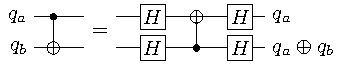
\includegraphics[scale=1]{fig/reverse}
}
\subcaptionbox{SWAP\label{fig:swap}}{
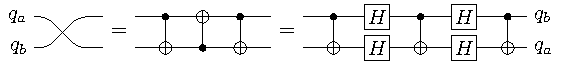
\includegraphics[scale=1]{fig/swap}
}
\caption{Allowed transformations}
\label{fig:transformations}
\end{figure}


Problem: find a valid implementation of the circuit that minimizes the number of swaps and CNOT reversals.

Note: the cost function is not obvious as algebraic simplifications can reduce the overhead of transformations.

\section{TODO}

\begin{itemize}
\item Express the quantum register allocation problem formally based on graph theory.
\item Assuming NP-completeness, reduce it to a known NP-complete problem.
\item Find an existing heuristic or propose a new one.
\item Collect some benchmarks.
\item Evaluate the heuristic against naive mapping and exact solution (which we can probably afford to compute for 5-qubit problems).
\item Profit!
\end{itemize}

%\section{The algorithm}

%\section{Conclusion}

\bibliographystyle{plain}
\bibliography{collange}



\end{document}
